% This chapter should discuss the global architecture of the whole app.
% It should not go into detail or implementation specifics.
% The chapters 'frontend', 'backend' and 'maintainability'
% should go into more detail and the implementation specifics.
%
% - Separation between domain, checks, RESTful server and frontend.
% - Checks as separated modules, but with the option to contact the domain.
% - Frontend with isolated elements and option to contact RESTful server and
%   checks.

The \gls{examiner} consists of four parts.
First of we have the domain we are working on, consisting of, among others,
% Hier verwijzen naar het domain model
tutors and students, the exercises, solutions
and the data that comprises these entities.
Secondly we have a control layer,
which acts as a separation between the domain layer and the application.
Then there are the various checks for investigating \gls{js-code}.
And finally, since we are dealing with a web application,
we have a distinct client side.
We will go into the details of each part in the sections below,
where we will discuss their part in the global architecture of the system,
and how the communication flows between each part.

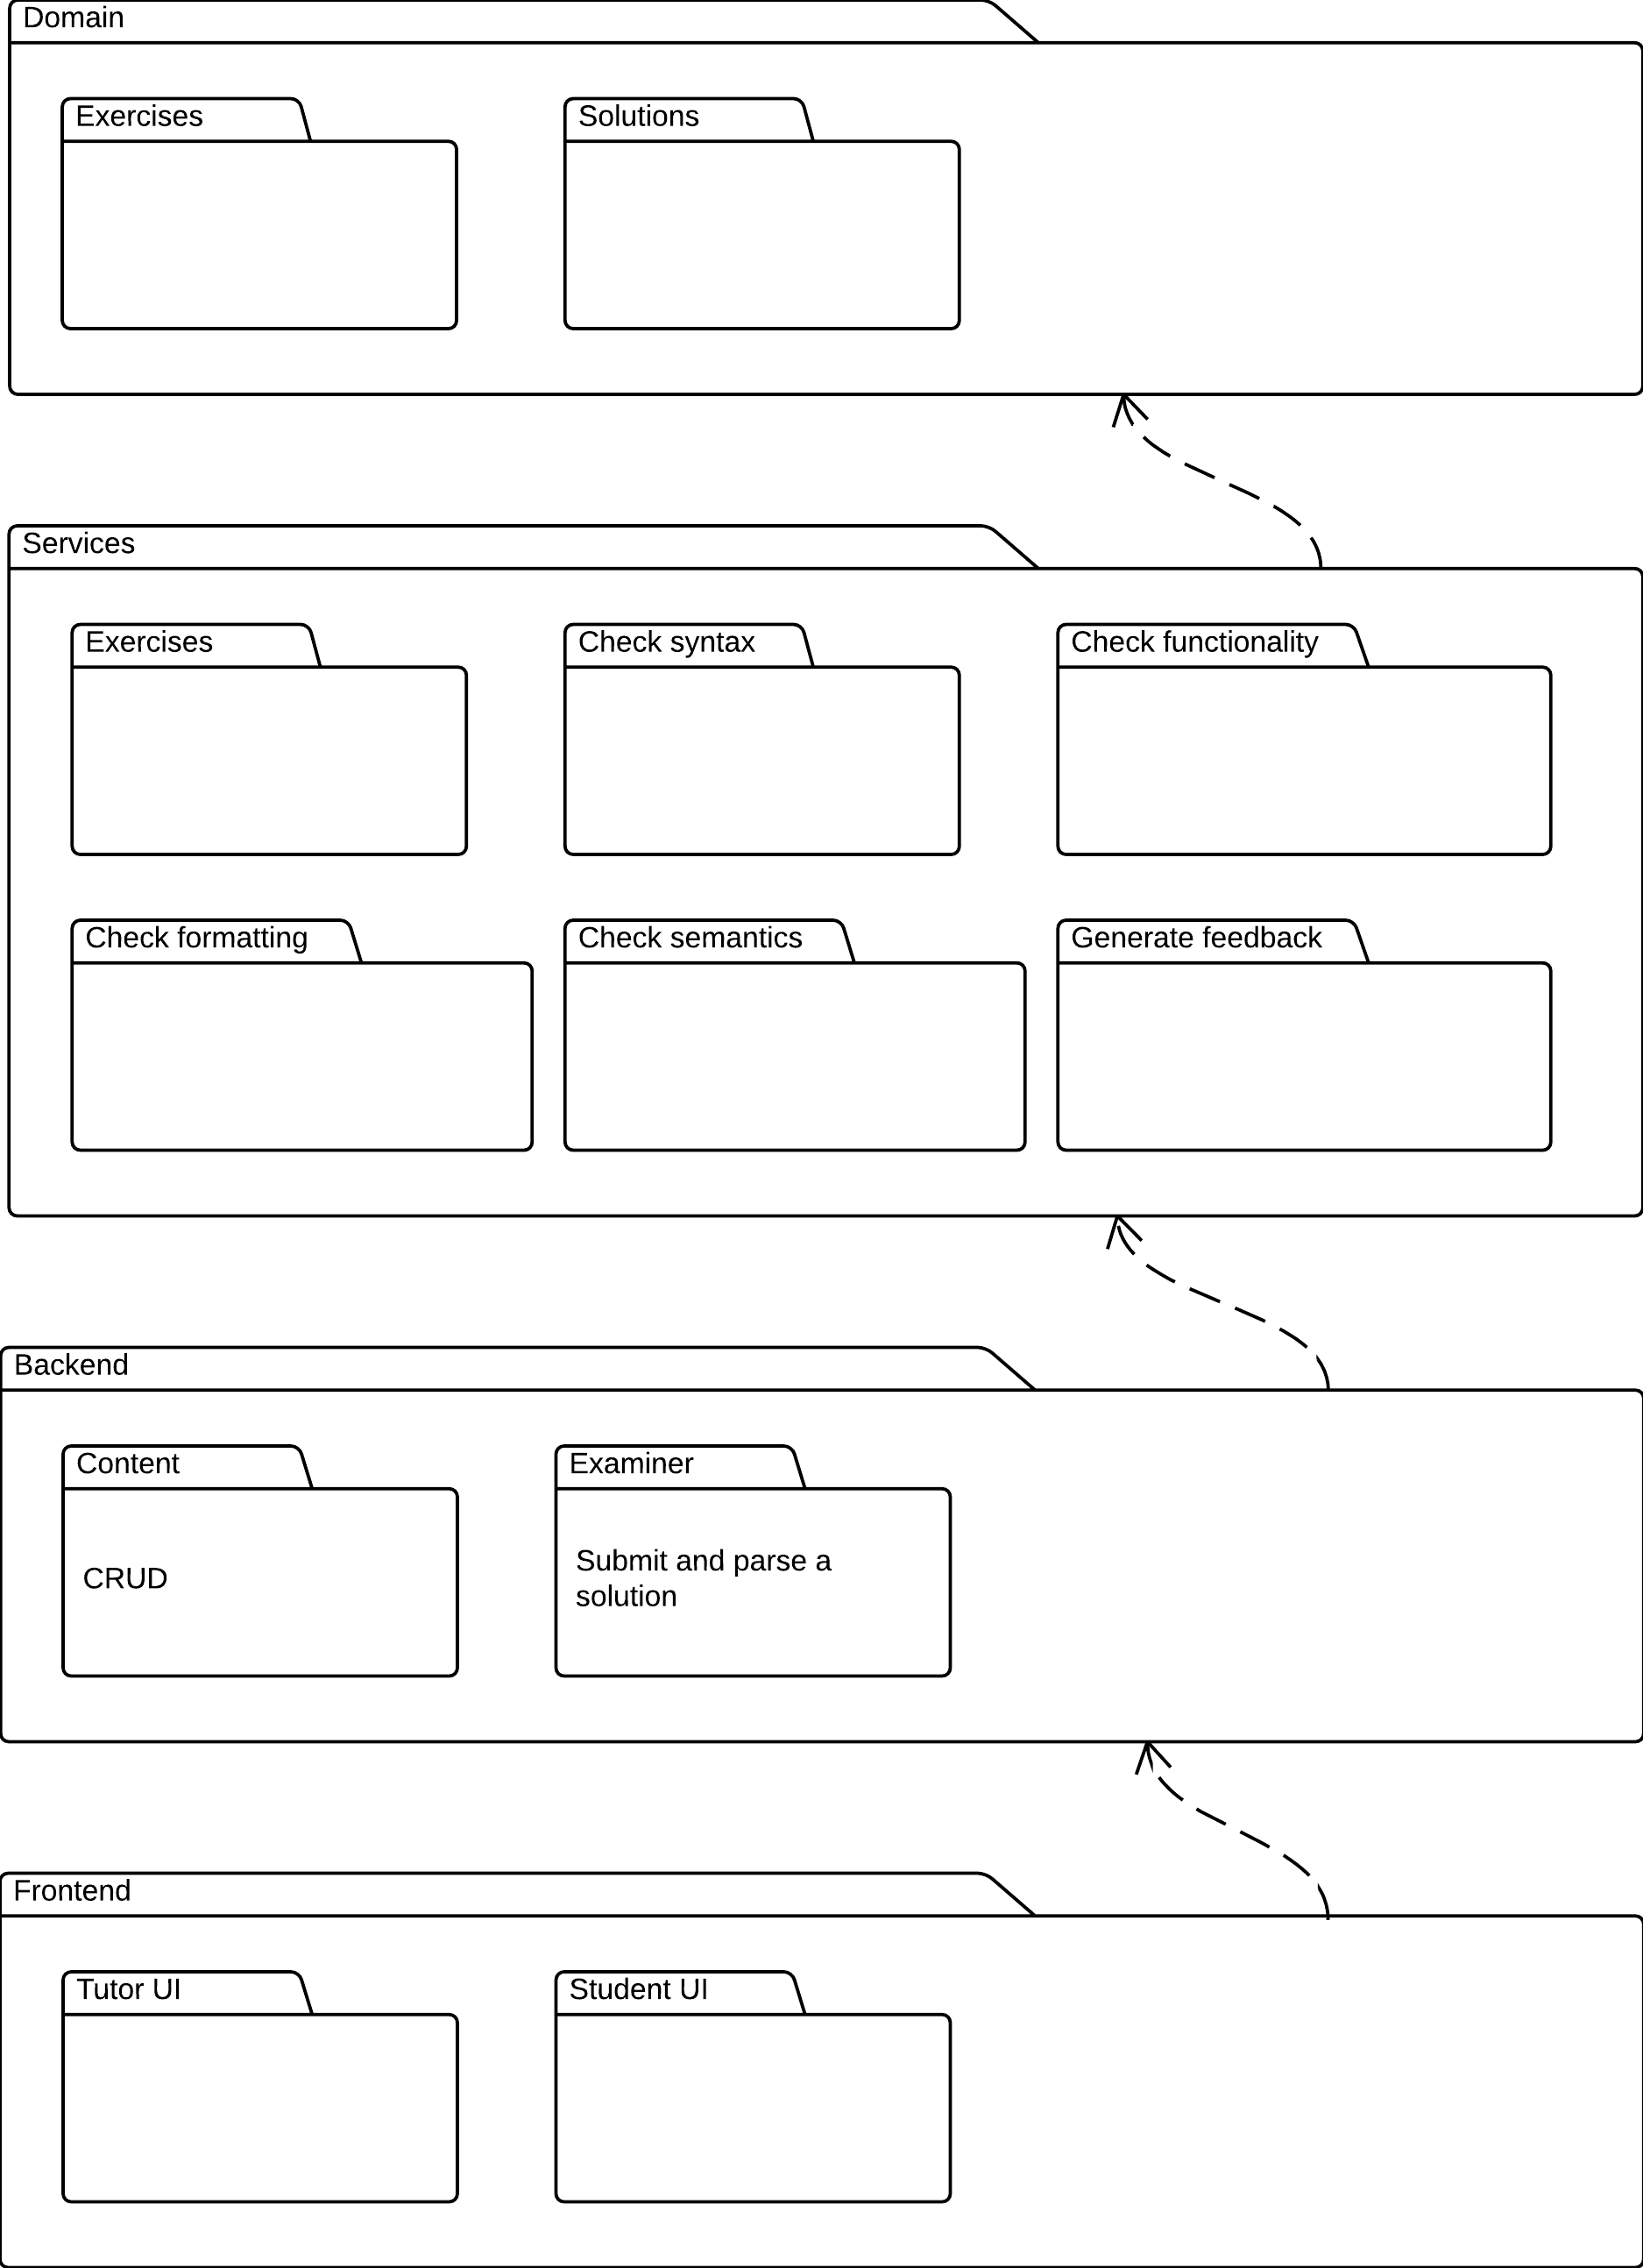
\includegraphics[scale=0.75]{diagrams-images/architecture}

\section{Control layer}
The control layer is the server side,
in the client-server architecture common to web applications.
It handles clientside requests
for retrieving or modifying a part of the domain.
Besides facilitating communication between the client side and the domain
it also does other things, like sending an email.

\section{Checks}
The checks are the modules that perform the examination of \gls{js-code}.
In order to make it easy to extend the system with more checks in the future
we placed the checks in relative isolation to the other parts of the system.
In the same way that the client communicates with the control layer,
the client can also communicate directly with each check.
Each check in its turn communicates back to the client
and can reach out to the domain if necessary.

As for the flow of the communication
the checks have the same place as the control layer.
In that manner they each are a specialized mini control layer on their own.
We deliberately pulled them apart from the cortrol layer though
in order to keep them as much plug-and-play as possible.
This way the checks are not limited
to the implementation we choose for the control layer.
While it is possible to place a check on the same server,
and write it in the same language as we choose for the control layer.
With this architecture it is certainly possible as well
to write the check in an other language
and even run it on a different server.

The only coupling the checks have is with the client and the domain.
The client controls the logic for contacting the various checks.
That logic would need to be updated when a check is added.
The checks also need access to the domain
and need to be able to access
the specific data storage implementation we choose for the domain.
The domain only needs to be altered if a check expands on the domain model.
This way the checks are decoupled from the control layer
and its implementation
which improves the ability to write,
and change the checks for the \gls{examiner}

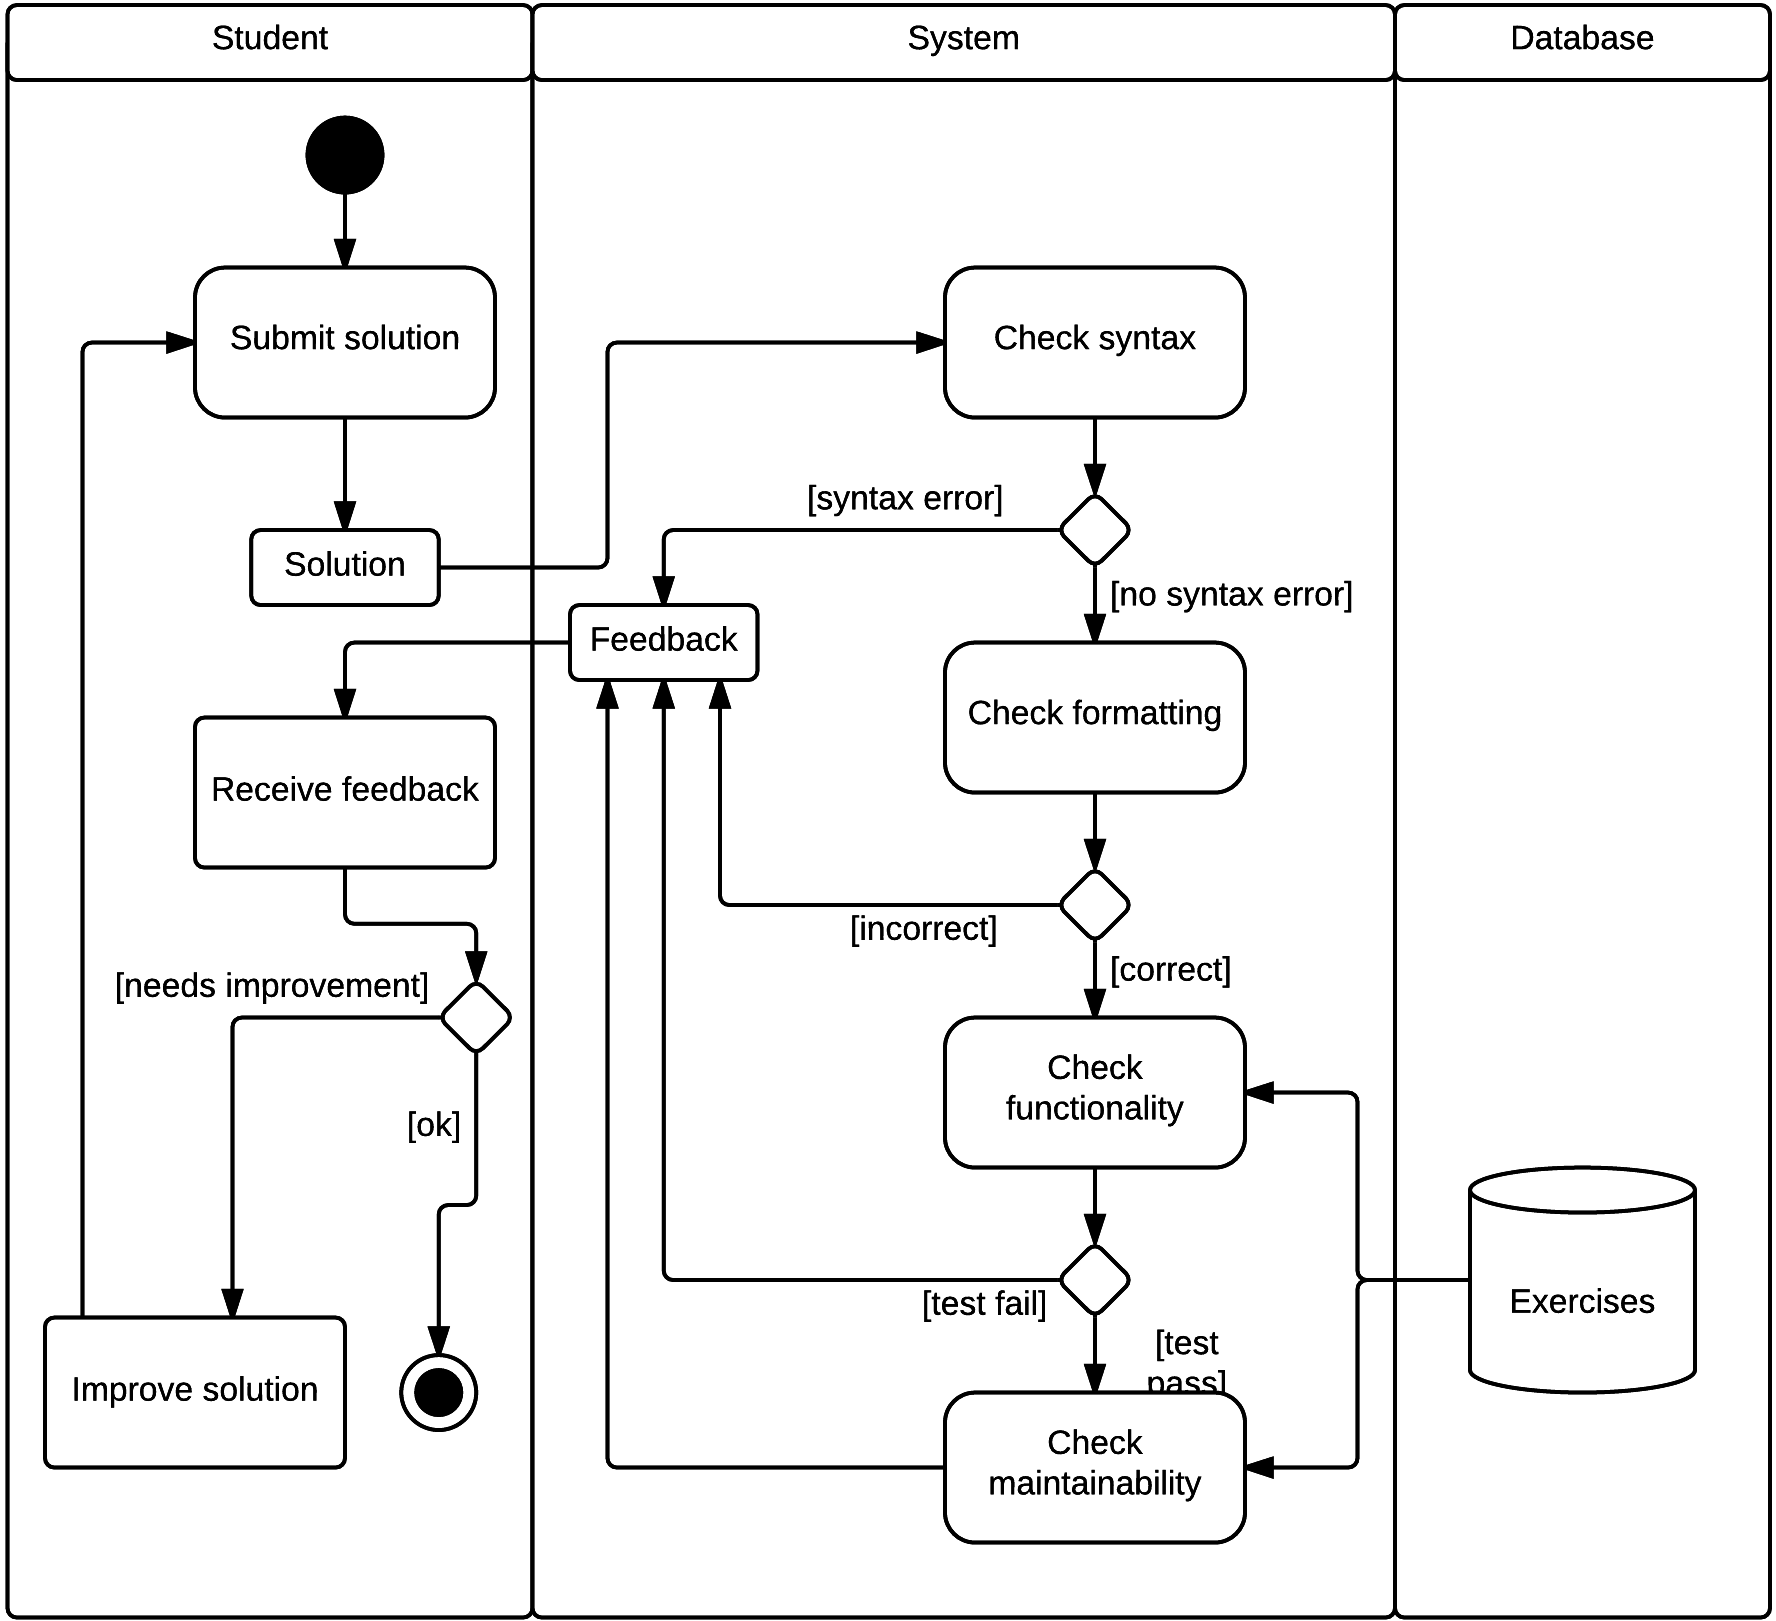
\includegraphics[scale=0.75]{diagrams-images/code-submission-activity-diagram}

\section{Client side}
Because we are building a web application
we have to deal with the browser side of things.
Thus we have a client side to our application.
To create a rich user experience we will a single page application.
No page reloads will occur
and communication with the server will be done through XHR requests.
The client will be responsible for the user interface
and the interaction with the user.
It will also carry out the logic directly coupled to the user interface.
For more domain specific logic
the client side will contact the control layer on the server side.
As well as for performing the various \gls{js-code} checks
the client side will contact the checks.

\section{Discussion}
We will be laying the groundwork for this project
with just a few of the functionalities it requires.
Other teams will pick up where we left and complement this software project.
Because of this we chose to use a service oriented approach.
Each functional requirement for examining \gls{js-code}
will be encapsulated in a service.
The backend \gls{source-code} has the ability to use these services.
It can call them in any order, use their responses
and supply responses from one service to another.
The frontend \gls{source-code} displays the user interface to the end user
and contacts the backend for sending and receiving the necessary information.
Persistence of data is managed through some kind of database system
containing the domain.
The backend has access to this domain.

For any future development of this project
the domain can be expanded
and services can be added
without the need to make complex changed to the existing code base.
Only the backend \gls{source-code} needs change
to make use of the added domain data and services.
